% !TEX root = paper.tex

\section{Algorithm} 
\label{sec:algorithm}

\subsection{Dimension Trees}
\label{sec:dimtrees}

An important optimization of the CP-ALS algorithm is to re-use temporary values across inner iterations \cite{PTC13a,KU16-TR,LCPSV17,Kaya17}.
To illustrate the idea, consider a 3-way tensor $\T{X}$ approximated by $\dsquare{\M{U},\M{V},\M{W}}$ and the two MTTKRP computations $\Mn{M}{1}=\underline{\Mz{X}{1}(\M{W}}\Khat\M{V})$ and $\Mn{M}{2}=\underline{\Mz{X}{2}(\M{W}}\Khat\M{U})$ used to update factor matrices $\M{U}$ and $\M{V}$, respectively.
The underlined parts of the expressions correspond to the shared dependence of the outputs on the tensor $\T{X}$ and the third factor matrix $\M{W}$.
Indeed, a temporary quantity, which we refer to as a \emph{partial MTTKRP}, can be computed and re-used across the two MTTKRP expressions.
We refer to the computation that combines the temporary quantity with the other factor matrix to complete the MTTKRP computation as a multi-tensor-times-vector or \emph{multi-TTV}, as it consists of multiple operations that multiply a tensor times a set of vectors, each corresponding to a different mode.
%This terminology was used in \cite{HBJT18}.

To understand the steps of the partial MTTKRP and multi-TTV operations in more detail, we consider $\T{X}$ to be $I\times J\times K$ and $\M{U}$, $\M{V}$, and $\M{W}$ to have $R$ columns.
Then 
\begin{equation*}
\MnE{M}{1}{ir} = \sum_{i,j} \TE{X}{ijk} \ME{V}{jr} \ME{W}{kr} 
= \sum_{j} \ME{V}{jr} \sum_k \TE{X}{ijk} \ME{W}{kr} 
= \sum_{j} \ME{V}{jr} \TE{T}{ijr},
\end{equation*}
where $\T{T}$ is an $I\times J\times R$ tensor that is the result of a partial MTTKRP between tensor $\T{X}$ and the single factor matrix $W$.
Likewise,
\begin{equation*}
\MnE{M}{2}{jr} = \sum_{i,k} \TE{X}{ijk} \ME{U}{ir} \ME{W}{kr} 
= \sum_{i} \ME{U}{ir} \sum_k \TE{X}{ijk} \ME{W}{kr} 
= \sum_{i} \ME{U}{ir} \TE{T}{ijr},
\end{equation*}
and we see that the temporary tensor $\T{T}$ can be re-used.
From these expressions, we can also see that computing $\T{T}$ (a partial MTTKRP) corresponds to a matrix-matrix multiplication, and computing each of $\Mn{M}{1}$ and $\Mn{M}{2}$ from $\T{T}$ (a multi-TTV) corresponds to $R$ independent matrix-vector multiplications.
In this case, we compute $\Mn{M}{3}$ using a full MTTKRP.

For a larger number of modes, a more general approach can organize the temporary quantities to be used over a maximal number of MTTKRPs.
The general approach can yield significant benefit, decreasing the computation by a factor of approximately $N/2$ for dense $N$-way tensors.
The idea is introduced in \cite{PTC13a}, but we adopt the terminology and notation of \emph{dimension trees} used for sparse tensors in \cite{KU16-TR,Kaya17}.
In this notation, the root node is labeled $\{1,\dots,N\}$ and corresponds to the original tensor, a leaf is labeled $\{n\}$ and corresponds to the $n$th MTTKRP result, and an internal node is labeled by a set of modes $\{i,\dots,j\}$ and corresponds to a temporary tensor whose values contribute to the MTTKRP results of modes $i,\dots,j$.

\begin{figure}
% !TEX root = ../paper.tex

\begin{center}
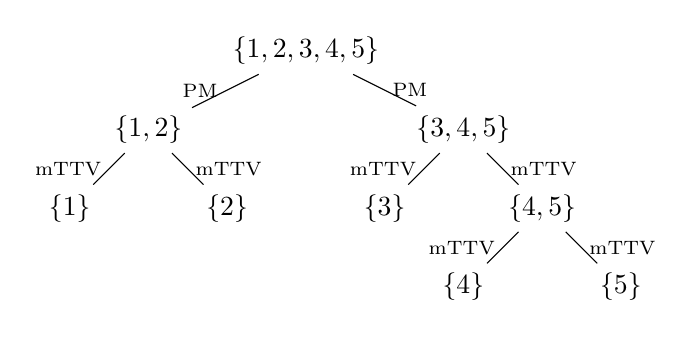
\begin{tikzpicture}

\node (12345) at (4,2) {$\{1,2,3,4,5\}$};
\node (12) at (2,1) {$\{1,2\}$};
\node (345) at (6,1) {$\{3,4,5\}$};
\node (1) at (1,0) {$\{1\}$};
\node (2) at (3,0) {$\{2\}$};
\node (3) at (5,0) {$\{3\}$};
\node (45) at (7,0) {$\{4,5\}$};
\node (4) at (6,-1) {$\{4\}$};
\node (5) at (8,-1) {$\{5\}$};

\scriptsize
\path[draw] (12345) edge [left,align=right] node {PM} (12);
\path[draw] (12345) edge [right,align=left] node {PM} (345);
\path[draw] (12) edge [left,align=right] node {mTTV} (1);
\path[draw] (12) edge [right,align=left] node {mTTV} (2);
\path[draw] (345) edge [left,align=right] node {mTTV} (3);
\path[draw] (345) edge [right,align=left] node {mTTV} (45);
\path[draw] (45) edge [left,align=right] node {mTTV} (4);
\path[draw] (45) edge [right,align=left] node {mTTV} (5);
\normalsize

\end{tikzpicture}
\end{center}
\caption{Dimension tree example for $N=5$. 
The data associated with the root node is the original tensor, the data associated with the leaf nodes are MTTKRP results, and the data associated with internal nodes are temporary tensors.  
Edges labeled with PM correspond to partial MTTKRP computations, and edges labeled with mTTV correspond to multi-TTV computations.}
\label{fig:DT}
\end{figure}

\Cref{fig:DT} illustrates a dimension tree for the case $N=5$.
Various shapes of binary trees are possible \cite{PTC13a,Kaya17}.
For dense tensors, the computational cost is dominated by the root's branches, which correspond to partial MTTKRP computations.
We perform the splitting of modes at the root so that modes are chosen contiguously with the respect to the layout of the tensor entries in memory.
In this way, each partial MTTKRP can be performed via BLAS's GEMM interface without reordering tensor entries in memory.
All other edges in a tree correspond to multi-TTVs and are typically much cheaper.
By organizing the memory layout of temporary quantities, the multi-TTV operations can be performed via a sequence of calls using BLAS's GEMV interface.
By using the BLAS in our implementation, we are able to obtain high performance and on-node parallelism.

\begin{figure}
\subfloat[Partial MTTKRP to compute node $\{3,4,5\}$ from root node $\{1,2,3,4,5\}$, executed via one GEMM call. \label{fig:DT-PM}]{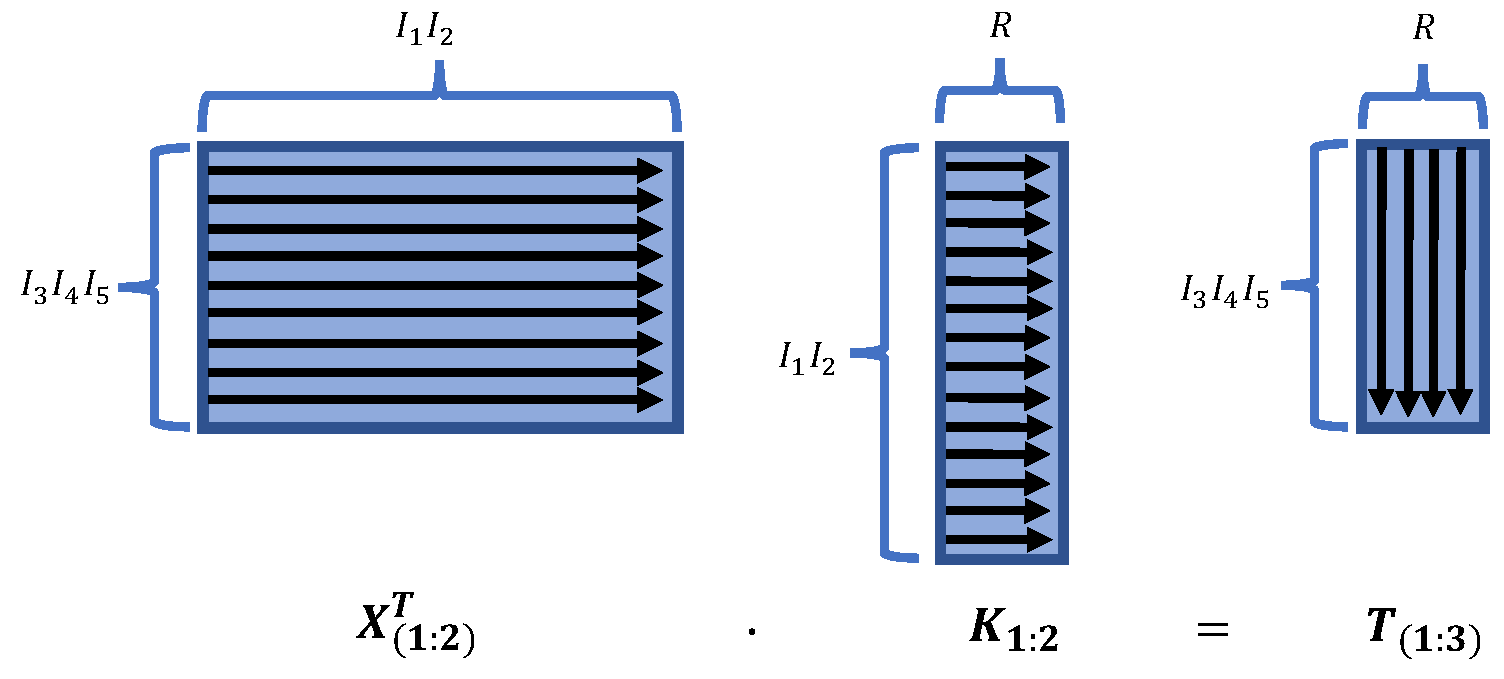
\includegraphics[width=\columnwidth]{fig/PM}} \\
\subfloat[Multi-TTV to compute node $\{3\}$ from node $\{3,4,5\}$, executed via $R$ GEMV calls.  Here $\Mz{T}{1} \lbrack r\rbrack$ refers to the $r$th contiguous block of $\Mz{T}{1}$. \label{fig:DT-mTTV}]{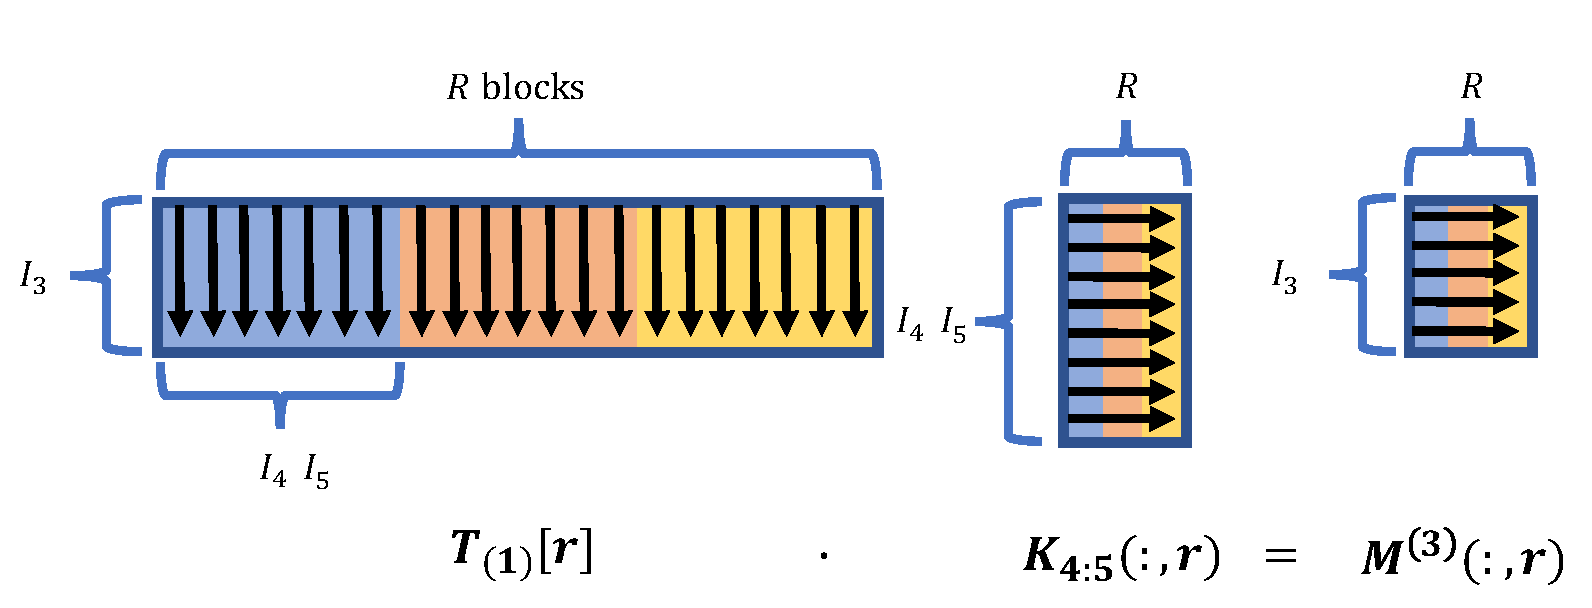
\includegraphics[width=\columnwidth]{fig/mTTV}}
\caption{Data layout and dimensions for two example computations in dimension tree shown in \Cref{fig:DT}.  In this notation, $\Mz{X}{3:5}$ is the matricization of input tensor $\T{X}$ with respect to modes 3 through 5, $\M{K}_{1:2} = \Mn{H}{2} \Khat \Mn{H}{1}$, $\T T$ is the temporary $I_3 \times I_4 \times I_5 \times R$ tensor corresponding to node $\{3,4,5\}$ in the dimension tree, $\M{K}_{4:5} = \Mn{H}{5} \Khat \Mn{H}{4}$, and $\Mn{M}{3}$ is the MTTKRP result for mode 3.}
\label{fig:DTcartoon}
\end{figure}

\Cref{fig:DTcartoon} shows the data layout and dimensions of a partial MTTKRP and a multi-TTV taken from the example dimension tree in \Cref{fig:DT}.
\Cref{fig:DT-PM} shows a partial MTTKRP between the input tensor $\T{X}$ and the Khatri-Rao product of the factor matrices in modes 1 and 2, which produces a temporary tensor $\T{T}$ corresponding to the $\{3,4,5\}$ node in the dimension tree.
The key to efficiency in this computation is that the matricization of $\T{X}$ that assigns modes 1 through 2 to rows and modes 3 through 5 to columns is already column-major in memory.
Thus, we can use the GEMM interface and compute the temporary tensor $\T{T}$ without reordering any tensor entries.
\Cref{fig:DT-mTTV} depicts a multi-TTV that computes the results $\Mn{M}{3}$ from $\T{T}$ and the factor matrices in modes 4 and 5.
Here, the tensor $\T{T}$ is matricized with respect to only its first mode (of dimension $I_3$), but this matricization is also column-major in memory.
We choose the ordering of the modes of $\T{T}$ such that each of $R$ contiguous blocks is used to compute one column of the output matrix via a matrix-vector operation with a corresponding column of the Khati-Rao product of the other factor matrices.

No matter how the dimension tree is designed, the computational cost of each partial MTTKRP is $O(IR)$, where $I$ is the number of tensor entries and $R$ is the rank of the CP decomposition.
This is the same operation count as a full MTTKRP.
The computational cost of a multi-TTV is the number of entries in the temporary tensor, which is the product of a \emph{subset} of the original tensor dimensions multiplied by $R$.
Thus, it is computationally cheaper than the partial MTTKRPs, but it is also memory bandwidth bound.

The other subroutine necessary for implementing the dimension tree approach is the Khatri-Rao product of sets of factor matrices.
We implement the operation as a row-wise Hadamard product of a set of factor matrix rows, and we use OpenMP parallelization to obtain on-node parallelism.
The computational cost of this operation is also typically lower order, but the running time in practice suffers from also being memory bandwidth bound.



\subsection{Relative Error Computation}
\label{sec:error}

Given a model $\T{M}=\CP$, we compute the relative error $\|\TA - \T{M}\|/\|\TA\|$ efficiently by using the identity $\|\TA-\T{M}\|^2 = \|\TA\|^2 - 2\langle \TA, \T{M} \rangle + \|\T{M}\|^2.$
The quantity $\|\TA\|$ is fixed, and the other two terms can be computed cheaply given the temporary matrices computed during the course of the BCD algorithm.
The second term can be computed using the identity $\langle \TA, \T{M} \rangle = \langle \Mn{M}{N}, \Mn{H}{N} \rangle$, where $\Mn{M}{N} = \Mz{A}{N} (\Mn{H}{N-1} \Khat \cdots \Khat \Mn{H}{1})$ is the MTTKRP result in the $N$th mode.
The third term can be computed using the identity $\|\T{M}\|^2 = \V{1}^\Tra(\Mn{S}{N} \Hada \MnTra{H}{N} \Mn{H}{N})\V{1}$ where $\Mn{S}{N}=\MnTra{H}{1} \Mn{H}{1} \Hada \cdots \Hada \MnTra{H}{N-1} \Mn{H}{N-1}$.
Both matrices $\Mn{M}{N}$ and $\Mn{S}{N}$ are computed during the course of the BCD algorithm for updating the factor matrix $\Mn{H}{N}$.
The extra computation involved in computing the relative error is negligible.
These identities have been used previously \cite{KB09,TensorBox,SK16,LKLHS2017}.

\subsection{Parallel Algorithm}

\begin{algorithm}
\caption{$\CP = \text{Par-NNCP}(\TA,R)$}
\label{alg:Par-NNCP-short}
\begin{algorithmic}[1]
\Require $\TA$ is an $I_1\times \cdots \times I_N$ tensor distributed across a $P_1\times \cdots \times P_N$ grid of $P$ processors, so that $\TA_{\V{p}}$ is $(I_1/P_1)\times \cdots \times (I_N/P_N)$ and is owned by processor $\V{p}=(p_1,\dots,p_N)$, $R$ is rank of approximation
\For{$n=2$ to $N$}
	\State Initialize $\Mn{H}{n}_{\V{p}}$ of dimensions $(I_n/P)\times R$ 
	\State $\M[\overline]{G} = \text{Local-SYRK}(\Mn{H}{n}_{\V{p}})$
	\State $\Mn{G}{n} = \text{All-Reduce}(\M[\overline]{G},\textsc{All-Procs})$
	\State $\Mn{H}{n}_{p_n} = \text{All-Gather}(\Mn{H}{n}_{\V{p}},\textsc{Proc-Slice}(n,\VE{p}{n}))$
\EndFor
\State \Comment{Compute NNCP approximation}
\While{not converged}
	\label{line:while}
	\State \Comment{Perform outer iteration of BCD}
	\For{$n=1$ to $N$}
		\label{line:for}
		\State \Comment{Compute new factor matrix in $n$th mode}
		\State $\M[\overline]{M} = \text{Local-MTTKRP}(\TA_{p_1\cdots p_N},\{\Mn{H}{i}_{p_i}\},n)$
			\label{line:locMTTKRP}
		\State $\Mn{M}{n}_{\V{p}} = \text{Reduce-Scatter}(\M[\overline]{M},\textsc{Proc-Slice}(n,\VE{p}{n}))$ 
			\label{line:reduce-scatter}
		\State $\Mn{S}{n} = \Mn{G}{1} \Hada \cdots \Hada \Mn{G}{n-1} \Hada \Mn{G}{n+1} \Hada \cdots \Hada \Mn{G}{N}$
			\label{line:hadamard}
		\State $\Mn{H}{n}_{\V{p}} = \text{Local-NLS-Update}(\Mn{S}{n},\Mn{M}{n}_{\V{p}})$
			\label{line:locNLS}
		\State \Comment{Organize data for later modes}
		\State $\M[\overline]{G} = {\Mn{H}{n}_{\V{p}}}^\Tra\Mn{H}{n}_{\V{p}}$
			\label{line:locSYRK}
		\State $\Mn{G}{n} = \text{All-Reduce}(\M[\overline]{G},\textsc{All-Procs})$
			\label{line:all-reduce}
		\State $\Mn{H}{n}_{p_n} = \text{All-Gather}(\Mn{H}{n}_{\V{p}},\textsc{Proc-Slice}(n,\VE{p}{n}))$
			\label{line:all-gather}
	\EndFor 
		\label{line:endfor}
\EndWhile
	\label{line:endwhile}
\Ensure $\TA \approx \CP$
\Ensure Local matrices: $\Mn{H}{n}_{\V{p}}$ is $(I_n/P)\times R$ and owned by processor $\V{p}=(p_1,\dots,p_N)$, for $1\leq n \leq N$, $\V{\lambda}$ stored redundantly on every processor
\end{algorithmic}
\end{algorithm}

\subsubsection{Algorithm Overview}

The basic sequential algorithm is given in \Cref{alg:nncp}, and the parallel version is given in \Cref{alg:Par-NNCP-short}.
We will refer to both the inner iteration, in which one factor matrix is updated (\cref{line:for} to \cref{line:endfor}), and the outer iteration, in which all factor matrices are updated (\cref{line:while} to \cref{line:endwhile}).
In the parallel algorithm, the processors are organized into a logical multidimensional grid (tensor) with as many modes as the data tensor.
The communication patterns used in the algorithm are all MPI collectives, including All-Reduce, Reduce-Scatter, and All-Gather.
The processor communicators (across which the collectives are performed) include the set of all processors and the sets of processors within the same processor slice.
Processors within a mode-$n$ slice all have the same $n$th coordinate.

The method of enforcing the nonnegativity constraints of the linear least squares solve (or update) generally affects only local computation because each row of a factor matrix can be updated independently.
In our algorithm, each processor solves the linear problem or computes the update for its subset of rows (see \cref{line:locNLS}). 
The most expensive (and most complicated) part of the parallel algorithm is the computation of the MTTKRP, which corresponds to \cref{line:locMTTKRP,line:reduce-scatter,line:all-gather}.

The details that are omitted from this presentation of the algorithm include the normalization of each factor matrix after it is computed and the computation of the residual error at the end of an outer iteration.
The computations do involve both local computation and communication, but their costs are negligible.
A more detailed pseudocode is given in \Cref{alg:Par-NNCP-long}.

% !TEX root = ../paper.tex

\newcommand{\procdim}{3}
\newcommand{\proc}{\draw[black,shift={(-.5,-.5)}] (0,0) grid (\procdim,\procdim);}
\newcommand{\highlight}{gray!75}
\newcommand{\commhighlight}{gray!25}
\newcommand{\parscale}{.46}
\newcommand{\secfaclabel}{$\Mn{M}{2}$}

\newcommand{\parbasepic}{
% highlight one processor's data
% front face
\begin{scope}[canvas is yz plane at x=.5,shift={(1.5,-1.5)}]
	% highlight front face of tensor block
	\draw[fill=\highlight,shift={(0,1)}] (0,0) rectangle (1,1);
	% highlight block of 1st factor matrix
	\draw[fill=\highlight,shift={(-2.5,2-1/3)},xscale=.5] (0,0) rectangle (-1,-1/9);
	% highlight block of 2nd factor matrix
	\draw[shift={(0,-1.5)},yscale=.5] (0,0) rectangle (1/9,-1);
\end{scope}
% right face
\begin{scope}[canvas is zx plane at y=(\procdim-.5),rotate=-90,shift={(-.5,-3)}]
	% highlight front face of tensor block
	\draw[fill=\highlight,shift={(0,2.5)}] (0,0) rectangle (1,1);
	% highlight block of 3rd factor matrix
	\draw[fill=\highlight,yscale=.5] (0,0) rectangle (1/9,-1);
\end{scope}
% top face
\begin{scope}[canvas is yx plane at z=.5,yscale=-1,rotate=0]
	% highlight front face of tensor block
	\draw[fill=\highlight,shift={(1.5,-.5)}] (0,0) rectangle (1,1);
\end{scope}

% draw tensor
% front face
\begin{scope}[canvas is yz plane at x=.5,rotate=-90]
	\proc
\end{scope}
% top face
\begin{scope}[canvas is yx plane at z=.5,yscale=-1,rotate=0]
	\proc
\end{scope}
% right face
\begin{scope}[canvas is zx plane at y=(\procdim-.5),rotate=180]
	\proc
\end{scope}

% draw factor matrices
% front face
\begin{scope}[canvas is yz plane at x=.5,shift={(1.5,-.5)}]
	% draw 1st factor matrix
	\draw[shift={(-2.5,0)},xscale=.5] (0,-2) grid (-1,1);
	\node[draw=none] at (-3.6,-.5) {\Large $\Mn{H}{1}$};
	% draw 2nd factor matrix
	\draw[shift={(0,-2.5)},yscale=.5] (-2,0) grid (1,-1);
	\node[draw=none] at (-.5,-3.5) {\Large \secfaclabel};
\end{scope}
% right face
\begin{scope}[canvas is zx plane at y=(\procdim-.5),rotate=-90,shift={(1.5,-.5)}]
	% draw 2nd factor matrix
	\draw[shift={(0,-2.5)},yscale=.5] (-2,0) grid (1,-1);
	\node[draw=none] at (-.5,-3.5) {\Large $\Mn{H}{3}$};
\end{scope}
}
\begin{figure*}[t]
\centering
  \subfloat[Start $n$th iteration with redundant subset of rows of each input matrix. \label{fig:inner_a}]{% !TEX root = Alg_header.tex

\begin{tikzpicture}[x={(-0.5cm,-0.4cm)}, y={(1cm,0cm)}, z={(0cm,1cm)},every node/.append style={transform shape},scale=\parscale]

% highlight all-gather/reduce-scatter patterns

% local computation
% front face
\begin{scope}[canvas is yz plane at x=.5]
	% highlight block of 1st factor matrix now owned by processor
	\draw[fill=\highlight,shift={(-1,.5)},xscale=.5] (0,0) rectangle (-1,-1);
\end{scope}
% right face
\begin{scope}[canvas is zx plane at y=(\procdim-.5),rotate=-90]
	% highlight block of 3rd factor matrix now owned by processor
	\draw[fill=\highlight,yscale=.5,shift={(-.5,-6)}] (0,0) rectangle (1,-1);
\end{scope}

% front face
\begin{scope}[canvas is yz plane at x=.5]
	% highlight block of 2nd factor matrix contribution computed by processor
	%\draw[fill=\highlight,shift={(1.5,-3)},yscale=.5] (0,0) rectangle (1,-1);
\end{scope}

\parbasepic

\end{tikzpicture}

}  \quad
  \subfloat[Compute local MTTKRP for contribution to output matrix $\Mn{M}{2}$. \label{fig:inner_b}]{% !TEX root = Alg_header.tex

\begin{tikzpicture}[x={(-0.5cm,-0.4cm)}, y={(1cm,0cm)}, z={(0cm,1cm)},every node/.append style={transform shape},scale=\parscale]

% highlight all-gather/reduce-scatter patterns

% local computation
% front face
\begin{scope}[canvas is yz plane at x=.5]
	% highlight block of 1st factor matrix now owned by processor
	\draw[fill=\highlight,shift={(-1,.5)},xscale=.5] (0,0) rectangle (-1,-1);
\end{scope}
% right face
\begin{scope}[canvas is zx plane at y=(\procdim-.5),rotate=-90]
	% highlight block of 3rd factor matrix now owned by processor
	\draw[fill=\highlight,yscale=.5,shift={(-.5,-6)}] (0,0) rectangle (1,-1);
\end{scope}

% front face
\begin{scope}[canvas is yz plane at x=.5]
	% highlight block of 2nd factor matrix contribution computed by processor
	\draw[fill=\highlight,shift={(1.5,-3)},yscale=.5] (0,0) rectangle (1,-1);
\end{scope}

\parbasepic

\end{tikzpicture}

}  \quad
  \subfloat[Reduce-Scatter to compute and distribute rows of $\Mn{M}{2}$. \label{fig:inner_c}]{% !TEX root = Alg_header.tex

\begin{tikzpicture}[x={(-0.5cm,-0.4cm)}, y={(1cm,0cm)}, z={(0cm,1cm)},every node/.append style={transform shape},scale=\parscale]

% highlight all-gather/reduce-scatter patterns
% reduce-scatter in 2nd mode

% front face
\begin{scope}[canvas is yz plane at x=.5]
	% highlight front face of proc comm
	\draw[fill=\commhighlight,shift={(1.5,.5)}] (0,0) rectangle (1,-3);
	% highlight block of 2nd factor matrix involved in reduce scatter
	\draw[fill=\commhighlight,shift={(1.5,-3)},yscale=.5] (0,0) rectangle (1,-1);
	% highlight block of 2nd factor matrix of computed output
	\draw[fill=\highlight,shift={(1.5,-3)},yscale=.5] (0,0) rectangle (1/9,-1);
	% highlight block of 1st factor matrix now owned by processor
	\draw[fill=\highlight,shift={(-1,.5)},xscale=.5] (0,0) rectangle (-1,-1);
\end{scope}
% right face
\begin{scope}[canvas is zx plane at y=(\procdim-.5),rotate=-90]
	% highlight right face of proc comm
	\draw[fill=\commhighlight,shift={(-.5,.5)}] (0,0) rectangle (3,-3);
	% highlight block of 3rd factor matrix now owned by processor
	\draw[fill=\highlight,yscale=.5,shift={(-.5,-6)}] (0,0) rectangle (1,-1);
\end{scope}
% top face
\begin{scope}[canvas is yx plane at z=.5,yscale=-1,rotate=0]
	% highlight top face of proc comm
	\draw[fill=\commhighlight,shift={(1.5,-.5)}] (0,0) rectangle (1,3);
\end{scope}

\parbasepic

\end{tikzpicture}

} \quad
  \subfloat[Compute local NLS update to obtain $\Mn{H}{2}_{\V{p}}$ from $\Mn{M}{2}_{\V{p}}$ (and $\Mn{S}{2}$). \label{fig:inner_d}]{% !TEX root = Alg_header.tex

\renewcommand{\secfaclabel}{$\Mn{H}{2}$}

\begin{tikzpicture}[x={(-0.5cm,-0.4cm)}, y={(1cm,0cm)}, z={(0cm,1cm)},every node/.append style={transform shape},scale=\parscale]

% highlight all-gather/reduce-scatter patterns
% reduce-scatter in 2nd mode

% front face
\begin{scope}[canvas is yz plane at x=.5]
	% highlight front face of proc comm
	%\draw[fill=\commhighlight,shift={(1.5,.5)}] (0,0) rectangle (1,-3);
	% highlight block of 2nd factor matrix involved in reduce scatter
	%\draw[fill=\commhighlight,shift={(1.5,-3)},yscale=.5] (0,0) rectangle (1,-1);
	% highlight block of 2nd factor matrix of computed output
	\draw[fill=\highlight,shift={(1.5,-3)},yscale=.5] (0,0) rectangle (1/9,-1);
	% highlight block of 1st factor matrix now owned by processor
	\draw[fill=\highlight,shift={(-1,.5)},xscale=.5] (0,0) rectangle (-1,-1);
\end{scope}
% right face
\begin{scope}[canvas is zx plane at y=(\procdim-.5),rotate=-90]
	% highlight right face of proc comm
	%\draw[fill=\commhighlight,shift={(-.5,.5)}] (0,0) rectangle (3,-3);
	% highlight block of 3rd factor matrix now owned by processor
	\draw[fill=\highlight,yscale=.5,shift={(-.5,-6)}] (0,0) rectangle (1,-1);
\end{scope}
% top face
\begin{scope}[canvas is yx plane at z=.5,yscale=-1,rotate=0]
	% highlight top face of proc comm
	%\draw[fill=\commhighlight,shift={(1.5,-.5)}] (0,0) rectangle (1,3);
\end{scope}

\parbasepic

\end{tikzpicture}

} \quad
  \subfloat[All-Gather to collect rows of $\Mn{H}{2}$ needed for later inner iterations. \label{fig:inner_e}]{% !TEX root = Alg_header.tex

\renewcommand{\secfaclabel}{$\Mn{H}{2}$}

\begin{tikzpicture}[x={(-0.5cm,-0.4cm)}, y={(1cm,0cm)}, z={(0cm,1cm)},every node/.append style={transform shape},scale=\parscale]

% highlight all-gather/reduce-scatter patterns
% reduce-scatter in 2nd mode

% front face
\begin{scope}[canvas is yz plane at x=.5]
	% highlight front face of proc comm
	\draw[fill=\commhighlight,shift={(1.5,.5)}] (0,0) rectangle (1,-3);
	% highlight block of 2nd factor matrix involved in reduce scatter
	\draw[fill=\highlight,shift={(1.5,-3)},yscale=.5] (0,0) rectangle (1,-1);
	% highlight block of 2nd factor matrix of computed output
	\draw[fill=\highlight,shift={(1.5,-3)},yscale=.5] (0,0) rectangle (1/9,-1);
	% highlight block of 1st factor matrix now owned by processor
	\draw[fill=\highlight,shift={(-1,.5)},xscale=.5] (0,0) rectangle (-1,-1);
\end{scope}
% right face
\begin{scope}[canvas is zx plane at y=(\procdim-.5),rotate=-90]
	% highlight right face of proc comm
	\draw[fill=\commhighlight,shift={(-.5,.5)}] (0,0) rectangle (3,-3);
	% highlight block of 3rd factor matrix now owned by processor
	\draw[fill=\highlight,yscale=.5,shift={(-.5,-6)}] (0,0) rectangle (1,-1);
\end{scope}
% top face
\begin{scope}[canvas is yx plane at z=.5,yscale=-1,rotate=0]
	% highlight top face of proc comm
	\draw[fill=\commhighlight,shift={(1.5,-.5)}] (0,0) rectangle (1,3);
\end{scope}

\parbasepic

\end{tikzpicture}

}
  \caption{Illustration of 2nd inner iteration of Par-NNCP algorithm for 3-way tensor on a $3\times3\times3$ processor grid, showing data distribution, communication, and computation across steps.  Highlighted areas correspond to processor $(1,3,1)$ and its processor slice with which it communicates.  The column normalization and computation of $\Mn{G}{2}$, which involve communication across all processors, is not shown here.}
  \label{fig:inner} 
\end{figure*}

\subsubsection{Data Distribution}
\label{sec:datadist}

Given a logical processor grid of processors $P_1\times \cdots \times P_N$, we distribute the tensor $\TA$ in a block or Cartesian partition.
Each processor owns a local tensor of dimensions $(I_1/P_1)\times \cdots \times (I_N/P_N)$, and only one copy of the tensor is stored.
Locally, the tensor is stored linearly, with entries ordered in a natural mode-descending way that generalizes column-major layout of matrices.
Given a processor $\V{p}=(\VE{p}{1},\dots,\VE{p}{N})$, we denote its local tensor $\TA_{\V{p}}$.

Each factor matrix is distributed across processors in a block row partition, so that each processor owns a subset of the rows.
We use the notation $\Mn{H}{n}_{\V{p}}$, which has dimensions $I_n/P\times R$ to denote the local part of the $n$th factor matrix stored on processor $\V{p}$.
However, we also make use a redundant distribution of the factor matrices across processors, because all processors in a mode-$n$ processor slice need access to the same entries of $\Mn{H}{n}$ to perform their computations.
The notation $\Mn{H}{n}_{\VE{p}{n}}$ denotes the $I_n/P_n\times R$ submatrix of $\Mn{H}{n}$ that is redundantly stored on all processors whose $n$th coordinate is $\VE{p}{n}$ (there are $P/P_n$ such processors).

Other matrices involved in the algorithm include $\Mn{M}{n}_{\V{p}}$, which is the result of the MTTKRP computation and has the same distribution scheme as $\Mn{H}{n}_{\V{p}}$, and $\Mn{G}{n}$, which is the $R\times R$ Gram matrix of the factor matrix $\Mn{H}{n}$ and is stored redundantly on all processors.

\subsubsection{Inner Iteration}

The inner iteration is displayed graphically in \Cref{fig:inner} for a 3-way example and an update of the $2$nd factor matrix.
The main idea is that at the start of the $n$th inner iteration (\cref{fig:inner_a}), all of the data is in place for each processor to perform a local MTTKRP computation.
This means that all processors in a slice redundantly own the same rows of the corresponding factor matrix (for all modes except $n$).
After the local MTTKRP is computed (\cref{fig:inner_b}), each processor has computed a contribution to a subset of the rows of the global MTTKRP $\Mn{M}{n}$, but its contribution must be summed up with the contributions of all other processors in its mode-$n$ slice.
This summation is performed with a Reduce-Scatter collective across the mode-$n$ processor slice that achieves a row-wise partition of the result (in \cref{fig:inner_c}, the light gray shading corresponds to the rows of $\Mn{M}{2}$ to which processor $(1,3,1)$ contributes and the dark gray shading corresponds to the rows it receives as output).
The output distribution of the Reduce-Scatter is designed so that afterwards, the update of the factor matrix in that mode can be performed row-wise in parallel.
Along with $\Mn{S}{n}$, which can be computed locally, each processor updates its own rows of the factor matrix given its rows of the MTTKRP result (\cref{fig:inner_d}).
The remainder of the inner iteration is preparing and distributing the new factor matrix data for future inner iterations, which includes an All-Gather of the newly computed factor matrix $\Mn{H}{n}$ across mode-$n$ processor slices (\cref{fig:inner_e}) and recomputing $\Mn{G}{n}={\Mn{H}{n}}^\Tra\Mn{H}{n}$.

\subsubsection{Analysis}

\begin{table*}
\centering
\begin{tabular}{|c|cccc|}
\hline
 & \textbf{Computation} & \textbf{Memory - Local MTTKRP} & \textbf{Communication} & \textbf{Memory - Par.~Algorithm}  \\
\hline
Par-NNCP w/ opt.~proc.~grid & $\frac{IR}{P}$ & $\frac{RI^{1/2}}{P^{1/2}}$& $\frac{NRI^{1/N}}{P^{1/N}}$ & $\frac{NRI^{1/N}}{P^{1/N}}$  \\
Par-NNCP w/ gen.~proc.~grid & & & $R\sum_n \frac{I_n}{P_n}$ & $R\sum_n \frac{I_n}{P_n}$  \\
Par-NNCP w/o dim.~tree opt. & $\frac{NIR}{P}$ & $\displaystyle \max_n \frac{RI/I_n}{P/P_n}$  &  & \\
\hline
\end{tabular}
\smallskip
\caption{Leading-order per-iteration costs in terms of computation (flops), communication (words moved), and memory (words).  We ignore constants but omit big-Oh notation for clarity.  The first line corresponds to \cref{alg:Par-NNCP-short} with an optimal choice of processor grid and applying the dimension tree optimization locally.  The second line corresponds to the changes in communication and memory for a general processor grid.  The third line corresponds to the changes in computation and memory if the dimension tree optimization is not applied.}
\label{tab:costs}
\end{table*}

We will analyze the cost of a single outer iteration.
While the number of outer iterations is sensitive to the NLS method used, the outer iteration time is generally the same across NLS methods.
We summarize the analysis in \cref{tab:costs}, showing the differences with and without an optimal processor grid and with and without using a dimension tree.

\paragraph{\emph{Computation}}
The local computation occurs at \cref{line:locMTTKRP,line:hadamard,line:locNLS,line:locSYRK}.
The cost of \cref{line:hadamard} is $O(NR^2)$, the cost of \cref{line:locNLS} is $O(R^3I_n/P)$, which is a loose upper bound for BPP and other methods \cite{KBP16}, and the cost of \cref{line:locSYRK} is $O(R(I_n/P)^2)$.
The sum of these three costs across all inner iterations is $O(R^2N^2+(R^3/P)\sum I_n+(R/P^2)\sum I_n^2)$, which is dominated by the cost of the MTTKRP.
When using dimension trees to perform the MTTKRP (\cref{line:locMTTKRP}), we compute the cost amortized over all inner iterations.
In this case, the cost is dominated by the two partial MTTKRP computations (from the root of the tree), which together are $O((R/P) \prod I_n)=O(IR/P)$ and dominate the costs of the multi-TTVs.
We note that this cost involves the product of all the tensor dimensions, which is why it dominates, and we note that it scales linearly with $P$.

\paragraph{\emph{Communication}}
The communication within the inner iteration occurs at \cref{line:reduce-scatter,line:all-reduce,line:all-gather}.
\Cref{line:all-reduce} involves $O(R^2)$ data and a collective across all processors.
\Cref{line:reduce-scatter,line:all-gather} involve $O(I_nR/P_n)$ data across a subset of $P/P_n$ processors.
Thus, the All-Reduce dominates the latency cost and the Reduce-Scatter/All-Gather dominate the bandwidth cost, for a total outer iteration communication cost of $O(R\sum I_n/P_n)$ words and $O(N\log P)$ messages.
If the optimal processor grid can be chosen to minimize communication (assuming $P$ is sufficiently factorable), then the bandwidth cost can achieve a value of $O(NRI^{1/N}/P^{1/N})$ by making the local tensors as cubical as possible.
We note that this cost scales with $P^{1/N}$, which is far from linear scaling.
However, it is proportional to the geometric mean of the tensor dimensions (on the order of one tensor dimension), which is much less than the computation cost dependence on the product of all dimensions.

\paragraph{\emph{Memory}}
The algorithm requires extra local memory to run.
Aside from the memory required to store the local tensor of $O(I/P)$ words and factor matrices of cumulative size $O((R/P)\sum I_n)$, each processor must be able to store a redundant subset of the rows of the factor matrices it needs to perform MTTKRP computations.
This corresponds to storing $P/P_n$ redundant copies of every factor matrix, which results in a local memory requirement of $O(R \sum I_n/P_n)$ for a general processor grid.
The processor grid that minimizes communication also minimizes local memory, and the extra memory requirement can be as low as $O(NRI^{1/N}/P^{1/N})$, which is typically dominated by $O(I/P)$.

The dimension tree algorithm also requires extra temporary memory space, but the space required tends to be much smaller than what is required to store the local tensor.
If the tensor dimensions can be partitioned into two parts with approximately equal geometric means, the extra memory requirement for running a dimension tree is as small as $O(R\sqrt{I/P})$, which is also typically dominated by $O(I/P)$.


